% This is text associated with the open textbook "Open Electromagnetics"
% See immediately below for author, date
% This work is licensed under the Creative Commons Attribution-ShareAlike 4.0 International License. (CC BY SA 4.0) 
% To view a copy of the license, visit http://creativecommons.org/licenses/by-sa/4.0/

%ORB TITLE Poynting's Theorem
%ORB AUTHOR 0        # S.W. Ellingson, Virginia Tech (ellingson@vt.edu)
%ORB DATE 20191119   # yyyymmdd
%ORB ABSTRACT 

\label{m0073_Poyntings_Theorem} % <-- Must match name of this file and module directory name.  Don't mess with this!
\index{Poynting's theorem|(}

Despite the apparent complexity of electromagnetic theory, there are in fact merely four ways that electromagnetic energy can be manipulated.
Electromagnetic energy can be:
%
\begin{itemize}
\item Transferred; i.e., conveyed  by transmission lines or in waves; 
\item Stored in an electric field (capacitance);
\item Stored in a magnetic field (inductance); or 
\item Dissipated (converted to heat; i.e., resistance).  
\index{Ohm's law}
\end{itemize}
%
Poynting's theorem is an expression of conservation of energy that elegantly relates these various possibilities.
Once recognized, the theorem has important applications in the analysis and design of electromagnetic systems.  
Some of these emerge from the derivation of the theorem, as opposed to the unsurprising result. 
So, let us now derive the theorem.

We begin with a statement of the theorem.  
Consider a volume $\mathcal{V}$ that may contain materials and structures in any combination.  
This is crudely depicted in Figure~\ref{m0073_fPT}.
%
\begin{figure}[b!] % <--- "[b]" for first figure in section *only*; delete for 2nd and subsequent figures
\begin{center}
\pdftooltip{{  % note double braces
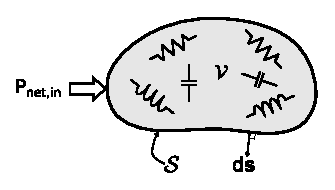
\includegraphics[width=2.5in]{modules/m0073_fPT.eps} 
% https://commons.wikimedia.org/wiki/File:Poynting%E2%80%99s_theorem_illustration.svg
}}{An arbitrarily shaped region capital V contains 2 unconnected resistors, capacitors, and inductors. Capital P subscript the quantity net comma in enters the region. The surface is capital S and a differential small d small s comes out of capital S perpendicular to region capital V.}
\end{center}
\centerline{\scriptsize 
\copyright~\hyperref[m0073_fPT_Credit]{C.\ Wang} 
\href{https://creativecommons.org/licenses/by-sa/4.0/}{CC BY-SA 4.0} 
} % \centerline 
\caption{
\label{m0073_fPT}
Poynting's theorem describes the fate of power entering a region $\mathcal{V}$ consisting of materials and structures capable of storing and dissipating energy.
}
\end{figure}
%  
Also recall that power is the time rate of change of energy.
Then:
%
\begin{equation}
P_{net,in} = P_E + P_M + P_{\Omega}
\label{m0073_ePTa}
\end{equation}
%
where 
$P_{net,in}$ is the net power flow into $\mathcal{V}$,
$P_E$ is the power associated with energy storage in electric fields within $\mathcal{V}$, 
$P_M$ is the power associated with energy storage in magnetic fields within $\mathcal{V}$, and
$P_{\Omega}$ is the power dissipated (converted to heat) in $\mathcal{V}$.

{\bf Some preliminary mathematical results.}  
We now derive two mathematical relationships that will be useful later.
Let ${\bf E}$ be the electric field intensity (SI base units of V/m) and let ${\bf D}$ be the electric flux density (SI base units of C/m$^2$).  
We require that the constituents of $\mathcal{V}$ be linear and time-invariant; therefore, ${\bf D}=\epsilon{\bf E}$ where the permittivity $\epsilon$ is constant with respect to time, but not necessarily with respect to position.
Under these conditions, we find
%
\begin{equation}
\frac{\partial}{\partial t} \left( {\bf E}\cdot{\bf D} \right)
= \frac{1}{\epsilon} \frac{\partial}{\partial t} \left( {\bf D}\cdot{\bf D} \right)
%\label{m0073_ePTp2a}
\end{equation}
%
Note that ${\bf E}$ and ${\bf D}$ point in the same direction.
Let $\hat{\bf e}$ be the unit vector describing this direction. 
Then, ${\bf E}=\hat{\bf e}E$ and ${\bf D}=\hat{\bf e}D$ where $E$ and $D$ are the scalar components of ${\bf E}$ and ${\bf D}$, respectively.  
Subsequently,
%
\begin{flalign}
\frac{1}{\epsilon} \frac{\partial}{\partial t} \left( {\bf D}\cdot{\bf D} \right)
 &= \frac{1}{\epsilon} \frac{\partial}{\partial t} D^2 \nonumber \\
 &= \frac{1}{\epsilon} 2D \frac{\partial}{\partial t} D \nonumber \\
 &= 2 {\bf E} \cdot \frac{\partial}{\partial t} {\bf D} 
\end{flalign}
%
Summarizing:
%
\begin{equation}
\frac{\partial}{\partial t} \left( {\bf E}\cdot{\bf D} \right)
= 2 {\bf E} \cdot \frac{\partial}{\partial t} {\bf D} 
\label{m0073_ePTp2}
\end{equation}
%
which is the expression we seek.  It is worth noting that the expressions on both sides of the equation have the same units, namely, those of power.

Using the same reasoning, we find:
%
\begin{equation}
\frac{\partial}{\partial t} \left( {\bf H}\cdot{\bf B} \right)
= 2 {\bf H} \cdot \frac{\partial}{\partial t} {\bf B} 
\label{m0073_ePTp3}
\end{equation}
%
where ${\bf H}$ is the magnetic field intensity (SI base units of A/m) and ${\bf B}$ is the magnetic flux density (SI base units of T).  

{\bf Derivation of the theorem.}  We begin with the differential form of Ampere's law:
\index{Ampere's law!general form}
%
\begin{equation}
\nabla \times {\bf H} = {\bf J} + \frac{\partial}{\partial t}{\bf D}
\end{equation}
%
Taking the dot product with ${\bf E}$ on both sides:
%
\begin{equation}
{\bf E} \cdot \left( \nabla \times {\bf H} \right) = {\bf E} \cdot {\bf J} + {\bf E} \cdot \frac{\partial}{\partial t}{\bf D} 
\label{m0073_ePTp3a} 
\end{equation}
%
Let's deal with the left side of this equation first.  
For this, we will employ a vector identity (Equation~\ref{m0140_edFxG}, Appendix~\ref{m0140_Vector_Identities}).  
This identity states that for any two vector fields ${\bf F}$ and ${\bf G}$,
%
\begin{equation}
\nabla \cdot \left( {\bf F} \times {\bf G} \right) 
= {\bf G} \cdot \left( \nabla \times {\bf F} \right)
- {\bf F} \cdot \left( \nabla \times {\bf G} \right)
\end{equation}
%
Substituting ${\bf E}$ for ${\bf F}$ and ${\bf H}$ for ${\bf G}$ and rearranging terms, we find
%
\begin{equation}
{\bf E} \cdot \left( \nabla \times {\bf H} \right)
= {\bf H} \cdot \left( \nabla \times {\bf E} \right)
- \nabla \cdot \left( {\bf E} \times {\bf H} \right) 
\label{m0073_ePTp4}
\end{equation}
%
Next, we invoke the Maxwell-Faraday equation:
\index{Maxwell-Faraday equation}
%
\begin{equation}
\nabla \times {\bf E} = -\frac{\partial}{\partial t}{\bf B}
\end{equation}
%
Using this equation to replace the factor in the parentheses in the second term of Equation~\ref{m0073_ePTp4}, we obtain:
%
\begin{equation}
{\bf E} \cdot \left( \nabla \times {\bf H} \right)
= {\bf H} \cdot \left( -\frac{\partial}{\partial t}{\bf B} \right)
- \nabla \cdot \left( {\bf E} \times {\bf H} \right) 
\end{equation}
%
Substituting this expression for the left side of Equation~\ref{m0073_ePTp3a}, we have
%
\begin{equation}
- {\bf H} \cdot \frac{\partial}{\partial t}{\bf B} 
- \nabla \cdot \left( {\bf E} \times {\bf H} \right) 
= {\bf E} \cdot {\bf J} + {\bf E} \cdot \frac{\partial}{\partial t} {\bf D}
\end{equation}
%
Next we invoke the identities of Equations~\ref{m0073_ePTp2} and \ref{m0073_ePTp3} to replace the first and last terms:
%
\begin{flalign}
- \frac{1}{2} \frac{\partial}{\partial t} \left( {\bf H}\cdot{\bf B} \right)
&- \nabla \cdot \left( {\bf E} \times {\bf H} \right) \nonumber \\
&= {\bf E} \cdot {\bf J} 
+ \frac{1}{2} \frac{\partial}{\partial t} \left(  {\bf E}\cdot{\bf D} \right)
\end{flalign}
%
Now we move the first term to the right-hand side and integrate both sides over the volume $\mathcal{V}$:
%
\begin{flalign}
- \int_{\mathcal{V}} &\nabla \cdot \left( {\bf E} \times {\bf H} \right) dv \nonumber \\
&= \int_{\mathcal{V}} {\bf E} \cdot {\bf J}~dv \nonumber \\
&+ \int_{\mathcal{V}} \frac{1}{2} \frac{\partial}{\partial t} \left( {\bf E}\cdot{\bf D} \right) dv \nonumber \\
&+ \int_{\mathcal{V}} \frac{1}{2} \frac{\partial}{\partial t} \left( {\bf H}\cdot{\bf B} \right) dv
\end{flalign}
%
The left side may be transformed into a surface integral using the divergence theorem: 
\index{divergence theorem}
%
\begin{equation}
\int_{\mathcal{V}} \nabla \cdot \left( {\bf E} \times {\bf H} \right) dv 
= \oint_{\mathcal{S}} \left( {\bf E} \times {\bf H} \right) \cdot d{\bf s}
\end{equation}
%
where $\mathcal{S}$ is the closed surface that bounds $\mathcal{V}$ and $d{\bf s}$ is the outward-facing normal to this surface, as indicated in Figure~\ref{m0073_fPT}.
Finally, we exchange the order of time differentiation and volume integration in the last two terms:
%
\begin{flalign}
- \oint_{\mathcal{S}} &\left( {\bf E} \times {\bf H} \right) \cdot d{\bf s} \nonumber \\
&= \int_{\mathcal{V}} {\bf E} \cdot {\bf J}~dv \nonumber \\
&+ \frac{1}{2}\frac{\partial}{\partial t} \int_{\mathcal{V}}  {\bf E}\cdot{\bf D}~dv \nonumber \\
&+ \frac{1}{2}\frac{\partial}{\partial t} \int_{\mathcal{V}}  {\bf H}\cdot{\bf B}~dv
\label{m0073_ePTi}
\end{flalign}
%
Equation~\ref{m0073_ePTi} is Poynting's theorem. 
Each of the four terms has the particular physical interpretation identified in Equation~\ref{m0073_ePTa}, 
as we will now demonstrate. 

{\bf Power dissipated by ohmic loss.} The first term of the right side of Equation~\ref{m0073_ePTi} is
%
\begin{equation}
\boxed{
P_{\Omega} \triangleq \int_{\mathcal{V}} {\bf E} \cdot {\bf J}~dv
}
\label{m0073_eJL}
\end{equation}
%
Equation~\ref{m0073_eJL} is \emph{Joule's law}.
\index{Joule's law}
%\footnote{See the section ``Power Dissipation in Conducting Media'' for a refresher.  This section may appear in a different volume depending on the version of the book you are reading.} 
Joule's law gives the power dissipated due to finite conductivity of material.  
The role of conductivity ($\sigma$, SI base units of S/m) can be made explicit using the relationship ${\bf J} = \sigma{\bf E}$
(Ohm's law)
\index{Ohm's law}
in Equation~\ref{m0073_eJL}, which yields:
%
\begin{equation}
P_{\Omega} = \int_{\mathcal{V}} {\bf E} \cdot \sigma {\bf E}~dv = \int_{\mathcal{V}} \sigma \left|{\bf E}\right|^2~dv
\end{equation}
%
$P_{\Omega}$ is due to the conversion of the electric field into conduction current, and subsequently into heat.
This mechanism is commonly known as \emph{ohmic loss} or \emph{joule heating}.  
\index{ohmic loss}
\index{joule heating}
It is worth noting that this expression has the expected units.
For example, in Equation~\ref{m0073_eJL},  ${\bf E}$ (SI base units of V/m) times ${\bf J}$ (SI base units of A/m$^2$) yields a quantity with units of W/m$^3$; i.e., power per unit volume, which is power density.
Then integration over volume yields units of W; hence, power. 
 
{\bf Energy storage in electric and magnetic fields.} The second term on the right side of Equation~\ref{m0073_ePTi} is: %may be rewritten as follows:
%
\begin{equation}
\boxed{
P_E \triangleq \frac{1}{2} \frac{\partial}{\partial t} \int_{\mathcal{V}} {\bf E}\cdot{\bf D}~dv
}
\label{m0073_ePE}
\end{equation}
%
Recall ${\bf D}=\epsilon{\bf E}$, where $\epsilon$ is the permittivity (SI base units of F/m) of the material.
Thus, we may rewrite the previous equation as follows:
%
\begin{flalign}
P_E &= \frac{1}{2} \frac{\partial}{\partial t} \int_{\mathcal{V}} {\bf E} \cdot \epsilon {\bf E}~dv \nonumber \\
    &= \frac{1}{2} \frac{\partial}{\partial t} \int_{\mathcal{V}} \epsilon \left|{\bf E}\right|^2~dv \nonumber \\
    &= \frac{\partial}{\partial t} \left( \frac{1}{2} \int_{\mathcal{V}} \epsilon \left|{\bf E}\right|^2~dv \right)
\end{flalign}
%
The quantity in parentheses is $W_e$, the energy stored in the electric field within $\mathcal{V}$.
%\footnote{See the section ``Electrostatic Energy'' for a refresher.  This section may appear in a different volume depending on the version of the book you are reading.}   
  
The third term on the right side of Equation~\ref{m0073_ePTi} is: 
%
\begin{equation}
\boxed{
P_M \triangleq \frac{1}{2} \frac{\partial}{\partial t} \int_{\mathcal{V}} {\bf H}\cdot{\bf B}~dv
}
\label{m0073_ePM}
\end{equation}
%
Recall ${\bf B}=\mu{\bf H}$, where $\mu$ is the permeability (SI base units of H/m) of the material.
Thus, we may rewrite the previous equation as follows:
%
\begin{flalign}
P_M &= \frac{1}{2} \frac{\partial}{\partial t} \int_{\mathcal{V}} {\bf H} \cdot \mu {\bf H}~dv \nonumber \\
    &= \frac{1}{2} \frac{\partial}{\partial t} \int_{\mathcal{V}} \mu \left|{\bf H}\right|^2~dv \nonumber \\
    &= \frac{\partial}{\partial t} \left( \frac{1}{2} \int_{\mathcal{V}} \mu \left|{\bf H}\right|^2~dv \right)
\end{flalign}
%
The quantity in parentheses is $W_m$, the energy stored in the magnetic field within $\mathcal{V}$.
%\footnote{See the section ``Magnetic Energy'' for a refresher.  This section may appear in a different volume depending on the version of the book you are reading.}   
 
{\bf Power flux through $\mathcal{S}$.} The left side of Equation~\ref{m0073_ePTi} is
%
\begin{equation}
\boxed{
P_{net,in} \triangleq -\oint_{\mathcal{S}} \left( {\bf E} \times {\bf H} \right) \cdot d{\bf s} 
}
\label{m0073_ePF}
\end{equation}
%
The quantity ${\bf E} \times {\bf H}$ is the \emph{Poynting vector},
\index{Poynting vector}
which quantifies the spatial power density (SI base units of W/m$^2$) of an electromagnetic wave and the direction in which it propagates.
The reader has likely already encountered this concept.
%\footnote{See the section ``Wave Power in a Lossless Medium'' for a refresher.  This section may appear in a different volume depending on the version of the book you are reading.} 
Regardless, we'll confirm this interpretation of the quantity ${\bf E} \times {\bf H}$ in Section~\ref{m0122_Poynting_Vector}.
For now, observe that integration of the Poynting vector over $\mathcal{S}$ as indicated in Equation~\ref{m0073_ePF} yields the total power flowing out of $\mathcal{V}$ through $\mathcal{S}$.
The negative sign in Equation~\ref{m0073_ePF} indicates that the combined quantity represents power flow \emph{in} to $\mathcal{V}$ through $\mathcal{S}$.  
Finally, note the use of a single quantity $P_{net,in}$ does \emph{not} imply that power is entirely inward-directed or outward-directed.
Rather, $P_{net,in}$ represents the \emph{net} flux; i.e., the \emph{sum} of the inward- and outward-flowing power.

{\bf Summary.}  Equation~\ref{m0073_ePTi} may now be stated concisely as follows:  
%
\begin{equation}
\boxed{
P_{net,in} = P_{\Omega} + \frac{\partial}{\partial t}W_e + \frac{\partial}{\partial t}W_m
}
\label{m0073_ePT}
\end{equation}
%
%%%%%%%%%%%%%%%%%%%%%%%%%%%%%%%%%%%%%%%%%%%%%%%
%ORB HIGHLIGHT
\begin{mdframed}[backgroundcolor=yellow!20,nobreak=true] 
Poynting's theorem (Equation~\ref{m0073_ePT}, with Equations~\ref{m0073_ePF}, \ref{m0073_eJL}, \ref{m0073_ePE}, and \ref{m0073_ePM})
states that the net electromagnetic power flowing into a region of space may be either dissipated, or used to change the energy stored in electric and magnetic fields within that region.  
\end{mdframed}
%%%%%%%%%%%%%%%%%%%%%%%%%%%%%%%%%%%%%%%%%%%%%%%
%
Since we derived this result directly from the general form of Maxwell's equations, these three possibilities are \emph{all} the possibilities allowed by classical physics, so this is a statement of conservation of power.  

Finally, note the theorem also works in reverse; i.e., the net electromagnetic power flowing \emph{out} of a region of space must have originated from some active source (i.e., the reverse of power dissipation) or released from energy stored in electric or magnetic fields. 

%%%%%%%%%%%%%%%%%%%%%%%%%%%%%%%%%%%%%%%%%

{\bf Additional Reading:}
\begin{itemize}
\item ``\href{https://en.wikipedia.org/wiki/Poynting_vector}{Poynting vector}'' on Wikipedia.
\end{itemize}

\index{Poynting's theorem|)}
